%%%%%%%%%%%%%%%%%%%%%%%%%%%%%%%%%%%%%%%%%%%%%%%%%%%%%%%%%%%%%%%%%%%%%%%%%%%%%%%%
%2345678901234567890123456789012345678901234567890123456789012345678901234567890
%        1         2         3         4         5         6         7         8

\documentclass[letterpaper, 10 pt, conference]{ieeeconf}  % Comment this line out if you need a4paper

%\documentclass[a4paper, 10pt, conference]{ieeeconf}      % Use this line for a4 paper

\IEEEoverridecommandlockouts                              % This command is only needed if
                                                          % you want to use the \thanks command

\overrideIEEEmargins                                      % Needed to meet printer requirements.

% See the \addtolength command later in the file to balance the column lengths
% on the last page of the document

% The following packages can be found on http:\\www.ctan.org
\usepackage{graphics} % for pdf, bitmapped graphics files
\usepackage{epsfig} % for postscript graphics files
%\usepackage{mathptmx} % assumes new font selection scheme installed
%\usepackage{times} % assumes new font selection scheme installed
\usepackage{amsmath} % assumes amsmath package installed
\usepackage{amssymb}  % assumes amsmath package installed
\usepackage{url}
\usepackage{subfigure}
% Rafael
\usepackage{xspace}
\usepackage{pgfplots}
\usepackage{graphicx}
\usepackage{epstopdf}
\usepackage{cite}
\usepackage{bm}


% axded by Rafael
%%%%%%%%%%%%%%%%%%%%%%%%%%%%%%%%%%%%%%%%%%%%%%%%%%%%%%%%%%%%%%%
\def\marhes{{\sc Marhes}\xspace}
\def\octor{{OctoRoACH}\xspace}
\def\octors{{OctoRoACHes}\xspace}
\def\turtle{{TurtleBot}\xspace}
\def\turtles{{TurtleBots}\xspace}
\newcommand{\ie}{{\it i.e.},\xspace}
\newcommand{\eg}{{\it e.g.},\xspace}
\newcommand{\cf}{{\it c.f.},\xspace}
\newcommand{\el}{{\it et al.},\xspace}
\newcommand{\etc}{\text{etc.}}

\providecommand{\norm}[1]{\left\lVert#1\right\rVert}

%% Math defs
% The set of reals, integers, etc.
\renewcommand{\Re}{\mathbb{R}}
\newcommand{\Ze}{\mathbb {Z}}
\newcommand{\Pe}{\mathbb {P}}
\newcommand{\I}{\mathcal{I}}

\newtheorem{definition}{Definition}
%%%%%%%%%%%%%%%%%%%%%%%%%%%%%%%%%%%%%%%%%%%%%%%%%%%%%%%%%%%%%%

\title{\LARGE \bf
Homework 4: The PCA and MUSIC algorithms
}

\author{Luis A. Valbuena Reyes% <-this % stops a speeeeace
%\thanks{*This work was not supported by the MAST project.}% <-this % stops a space
\thanks{Luis Valbuena is with the Department of Electrical and Computer Engineering,
        University of New Mexico, Albuquerque, NM, 87131-0001, {\tt\small \{lavalbuenar@unm.edu\}}}%
}

\begin{document}

\newtheorem{theoremMyThesis}{Theorem}
\newtheorem{corollary}{Corollary}
\newtheorem{problemStatement}{Problem Statement}

\maketitle
\thispagestyle{empty}
\pagestyle{empty}


%%%%%%%%%%%%%%%%%%%%%%%%%%%%%%%%%%%%%%%%%%%%%%%%%%%%%%%%%%%%%%%%%%%%%%%%%%%%%%%%
\begin{abstract}

In this document, we present the solution for homework 4. Trying to follow the guidelines for writing papers, we develop each the requirements of the assignment on Sections \ref{sec:Theory}, \ref{sec:Experiments}, and \ref{sec:Conclusion}.
\end{abstract}

%%%%%%%%%%%%%%%%%%%%%%%%%%%%%%%%%%%%%%%%%%%%%%%%%%%%%%%%%%%%%%%%%%%%%%%%%%%%%%%%


\section{INTRODUCTION}
\label{sec:Intro}



%%%%%%%%%%%%%%%%%%%%%%%%%%%%%%%%%%%%%%%%%%%%%%%%%%%%%%%%%%%%%%%%%%%%%%%%%%%%%%%%


\section{Theory}
\label{sec:Theory}

We want to explain an observed variable $x_{i}$ with a variable $z_{i}$ through a Gaussian distribution. This time, we include 
a rotation, dilation and translation in the form

\begin{equation*}
   x_{i} , \leftarrow \bm{W}z_{i} + \bm{\mu}.
\end{equation*}

At the same time, with the matrix $\bm{W}$ we can discard the dimensions of a particular signal which do not pose a significant contribution to the composition
of the signal. That is Principal Component Analysis: determine which dimensions (components) are truly important in the representation of a signal. There are
two approach.

\subsection{Basic PCA}
\label{sec:TheoryBasicPCA}

The MUSIC power spectrum is given by:

\begin{equation*}
    S^{MUSIC}(k) = \frac{1}{\bm{e}_{k}^{H} R^{-1}\bm{e}_{k} },
\end{equation*}
which after discarding the signal eigenvectors to achieve perpendicularity and at the same time a singularity on the expression, we have
\begin{equation*}
    S^{MUSIC}(k) = \frac{1}{\bm{e}_{k}^{H} \bm{V}_{n}  \bm{V}_{n}^{H}\bm{e}_{k} },
\end{equation*}
where $\bm{e}_{k}  = [ 1 \exp{(j\omega_{k})}, \hdots, \exp{(j(L-1)\omega_{k})} ]$. We embed the observed variable in $\bm{e}_{k} $.

To obtain an equivalent MUSIC power spectrum using the signal eigenvectors, and based on the descomposition of matrix $ \bm{V} = [ \bm{V}_{s}  \bm{V}_{n}]$we start with the expression:

\begin{equation*}
    \bm{V}\bm{V}^{H} = \bm{V}_{s}\bm{V}_{s}^{H} + {V}_{n}\bm{V}_{n}^{H} = \bm{I},
\end{equation*}
where the dimensions of all the product matrices are the same. Solving for ${V}_{n}\bm{V}_{n}^{H} =  \bm{I} -  \bm{V}_{s}\bm{V}_{s}^{H}$, we obtain

\begin{equation*}
    S^{MUSIC \prime}(k) = \frac{1}{\bm{e}_{k}^{H}(\bm{I} -  \bm{V}_{s}\bm{V}_{s}^{H})\bm{e}_{k} },
\end{equation*}

The depiction of the two expression is presented in Fig.~\ref{fig:PowerSpectrum}.

\subsection{Probabilistic PCA}
\label{sec:TheoryProbabilisticPCA}

In contrast to the basic PCA, there is an iterative process based on the Expectation Maximization. The algorithm is

\begin{enumerate}
\item Initialize $W$.
\item $Z = (W^{H}W)^-1 W^{H}X$.
\item $W_{p} = XZ^{H}(ZZ^{H})^{-1}$.
\item $W_{pp} = W_{p}W_{p}^{H}RW_{p}$. 
\item $W = \text{gramschmidt}(W_{pp})$.
\item $\Lambda = W^{H}RW$.
\item Go to 1).
\end{enumerate}
where the function $\text{gramschmidt}(\ast)$ transform a nonsingular matrix (request also well-conditioned matrix) into an orthonormal form.

%%%%%%%%%%%%%%%%%%%%%%%%%%%%%%%%%%%%%%%%%%%%%%%%%%%%%%%%%%%%%%%%%%%%%%%%%%%%%%%%


\section{Experiments}
\label{sec:Experiments}

In a set of $D$ antennas, a snapshot $x[n]$ is received. Our purpose is to find the angle of the source of such a signal. The code for the generation of 
the artificially generated data is given on the assignment. We need to generate $100$ samples of the data where we embed the source angles 
$\theta_{1} = \pi/2$,  $\theta_{2} = \pi$, and $\theta_{3} = 3\pi/2$. The amplitude of the signals were chosen arbitrarily to be $A_{1} = 5.2$,  $A_{2} = 3.5$, 
and $A_{3} = 2.7$.

\subsection{Basic PCA}
\label{sec:ExperimentsBasicPCA}

There is a sequence of steps to implement the standard PCA algorithm and test it into the MUSIC algorithm: After generating the data as explained above, 
we compute the autocorrelation matrix of the data, all the eigenvectors and we compute the inverse of the power spectrum of the noise eigenvectors, which is
depicted in Fig.~\ref{fig:MUSICNOISEEIGENVECTORS}.

\begin{figure}[ht!]
 \begin{center}
  	\subfigure[\label{fig:MUSICNOISEEIGENVECTORS}]{\includegraphics[width=0.46\textwidth,trim=5 15 5 1]{Drawings/MUSICNOISEEIGENVECTORS.eps}}
 	\subfigure[\label{fig:MUSICSIGNALEIGENVECTORS}]{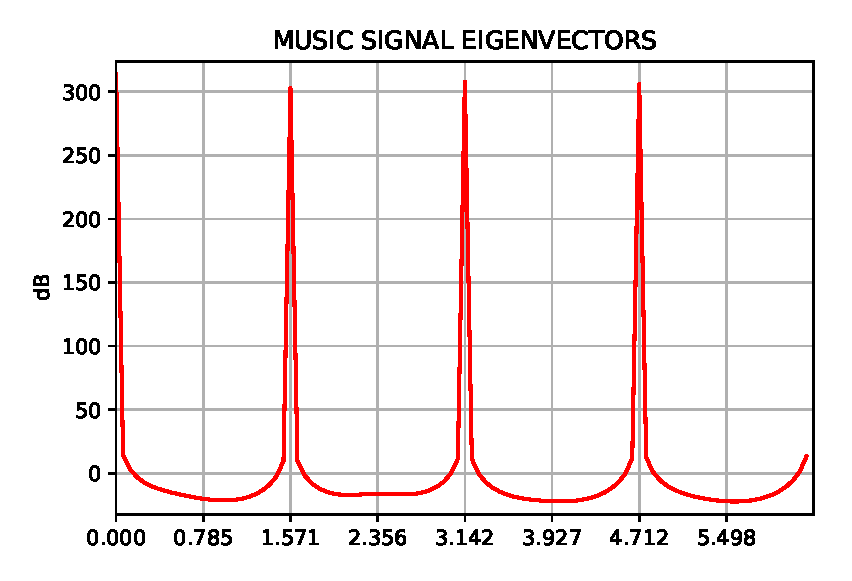
\includegraphics[width=0.46\textwidth,trim=5 5 5 1]{Drawings/MUSICSIGNALEIGENVECTORS.eps}}
         \caption{MUSIC Power Spectrum using  (a) noise eigenvectors, (b) signal eigenvectors. }
 \label{fig:PowerSpectrum}
 \end{center}
\end{figure}

\subsection{Probabilistic PCA}
\label{sec:ExperimentsProbabilisticPCA}

We initialize $\bm{W}$ as an identity matrix for the algorithm described in Section \ref{sec:TheoryProbabilisticPCA}.

\begin{equation*}
\lambda_{PPCA} = \begin{bmatrix}
 4696.6967 + 0j\\
 3938.0821 +3.4106e-13j\\
 3898.0878 +2.2737e-13j\\
 1033.6755 +1.4210e-14j\\
 1071.7745 +1.4210e-14j\\
  296.8125 -4.2632e-14j\\
  291.1196 +7.10546e-14j\\
 4053.5474 -1.1368e-13j\\
 1281.6756 +4.2632e-14j\\
  510.0582 +8.5265e-14j\end{bmatrix}
   \end{equation*}.
  
In contrast, the eigenvalues reported from the basic PCA are

\begin{equation*}
\lambda_{signal} = \begin{bmatrix}
4709.4496 -5.2921e-15j\\   
510.5888 -2.16221e-14j\\
   211.3332 -4.6848e-14j\\   
   148.5890 +8.6841e-14j\end{bmatrix}.
\end{equation*}

\begin{equation*}
\lambda_{noise} = \begin{bmatrix}
-2.9908e-13 +1.4491e-14j\\  
9.3037e-14 -5.2206e-14j\\
   7.3982e-14 +3.2462e-14j\\ 
    -7.4499e-14 -1.9217e-14j\\
   2.5000e-14 -1.9694e-15j\\  
   -3.5562e-14 +2.38656e-14j\end{bmatrix}.
\end{equation*}

where evidently there is not a visible relationship between the eigenvalues reported from the basic PCA and the probabilistic approach. 
%%%%%%%%%%%%%%%%%%%%%%%%%%%%%%%%%%%%%%%%%%%%%%%%%%%%%%%%%%%%%%%%%%%%%%%%%%%%%%%%

\section{Conclusion}
\label{sec:Conclusion}

In this final assignment, we took the problem of detecting the origin of a signal using an array of antennas. The goal is to confront the two approaches of PCA: the basic PCA and
the probabilistic PCA.

The results obtained on the  probabilistic PCA are dubious. We are concerned with line 6) of the algorithm presented on Section \ref{sec:TheoryProbabilisticPCA}
\begin{equation*}
\begin{aligned}
\bm{\Lambda} & = \bm{W}^{H} \bm{R} \bm{W},\\
              & = \bm{\Lambda}^{H} \bm{V}^{H} \bm{V} \bm{\Lambda} \bm{V}^{H} \bm{V} \bm{\Lambda},\\
              & = \bm{\Lambda} \bm{\Lambda} \bm{\Lambda}?,\\
\end{aligned}
\end{equation*}
 
% \subsection{SVM for Regression}
%\label{sec:ConclusionSVMRegression}


%%%%%%%%%%%%%%%%%%%%%%%%%%%%%%%%%%%%%%%%%%%%%%%%%%%%%%%%%%%%%%%%%%%%%%%%%%%%%%%%

%References are important to the reader; therefore, each citation must be complete and correct. If at all possible, references should be commonly available publications.


%\pagebreak

\bibliographystyle{IEEEtran}
\bibliography{References}

%%%%%% APPENDIX %%%%%%%
%q\input{Appendix}
\end{document}
